\chapter{Das LHCb-Experiment}
Der Large Hadron Collider (LHC) am Kernforschungszentrum CERN in Genf ist der derzeit größte Ringbeschleuniger der Erde. Er hat einen Durchmesser von ca. $27\kilo\meter$. Im Ring werden zwei geladene Teilchenstrahlen in gegenläufiger Richtung auf nahezu Lichtgeschwindigkeit beschleunigt und anschließend an vier möglichen Punkten zur Kollision gebracht. Bei den Teilchenstrahlen handelt es sich hauptsächlich um Protonenstrahlen, es werden aber auch Proton-Blei- und Blei-Blei-Kollisionen untersucht. An den vier Kollisionspunkten sind die großen Experimente positioniert: ATLAS, CMS, ALICE und LHCb. Eine der Hauptaufgaben der Experimente ATLAS und CMS ist die Suche nach dem Higgs-Boson, ALICE hingegen untersucht das Quark-Gluon-Plasma. Im folgenden soll nun aber detailliert auf das LHCb-Experiment eingegangen werden. \cite{lhc-info}
\section{Aufgaben und Ziele des Experimentes}
Während des Urknalls sind Materie und Antimaterie in gleicher Zahl entstanden. Triffen ein Teilchen und ein Antiteilchen aufeinander, so werden diese vernichtet und es wird Energie frei. Doch wenn zunächst gleich viel Materie und Antimaterie vorhanden war, verwundert es, warum das Universum nur aus Materie besteht und überhaupt noch existiert.

Das Standardmodell der Teilchenphysik kann dieses Ungleichgewicht nur unzureichend erklären. Es beschreibt zwar die \CP-Verletzung der schwachen Wechselwirkung, die auch Bestandteil dieser Arbeit ist, und liefert damit einen potentiellen Kandidaten zur Erkärung, allerdings jene zu schwach. Es muss also auch \CP-verletzende Beiträge jenseits des Standardmodells geben. Genau dieser Frage hat sich LHCb (Large Hadron Collider beauty) verschrieben. Es untersucht Teilchen und Zerfälle, die von einem $b$- bzw. $\overline{b}$-Quark (außerdem auch $c/\overline{c}$-Quarks) ausgehen. Aus diesen bilden sich B-(D-)Mesonen, die sehr sensitiv auf Hinweise für \glqq neue Physik\grqq\ sind. In diversen Zerfalls- und Mischprozessen enthalten die dazugehörigen Feynmangraphen Schleifen, in denen es möglich ist, dass neben dem Standardmodell auch \glqq neue Physik\grqq\ Beiträge zu Zerfallsamplituden etc. liefert. Man versucht also indirekt Hinweise auf neue Teilchen und Prozesse zu finden. Um dies erfolgreich zu gestalten, ist eine präzise Messung des Standardmodells unabdingbar. \cite{lhcb-info}

\section{Der LHCb-Detektor}
Im Gegensatz zu den anderen Experimenten ist der LHCb-Detektor ein einarmiger Vorwärtsspektrometer. Dies liegt daran, dass $b\overline{b}$-Paare hauptsächlich in oder entgegen der Protonenstrahlrichtung produziert werden. Aus Kostengründen hat man darauf verzichtet, den Detektor in Vorwärts- und Rückwärtsrichtung zu bauen. Stattdessen lag der Fokus darauf, nur einen Detektor, aber mit entsprechend besserer Präzision und Auflösung zu bauen. Abbildung \ref{fig:detektor} zeigt einen Schnitt durch die (y,z)-Ebene des Detektors. Der Detektor deckt in x-Richtung einen Bereich von $10-300\milli\rad$ und in y-Richtung von $10-250\milli\rad$ ab. Die Subdetektoren lassen sich nach ihrem Zweck in zwei Unterkategorien einteilen: Detektoren zur Spurrekonstruktion und zur Teilchenidentifikation.

\begin{figure}[hptb]
\centering
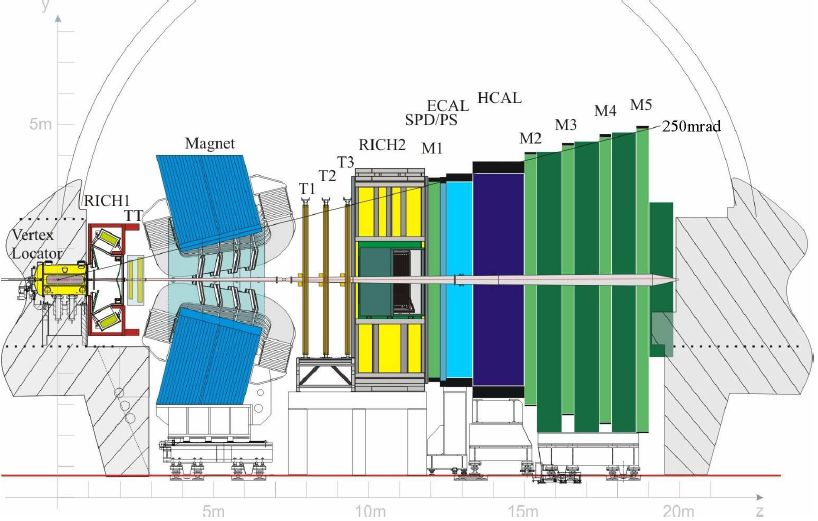
\includegraphics[width=\textwidth]{detektor}
\caption{Schnitt durch die (y,z)-Ebene des LHCb-Detektors. Die Abbildung wurde \cite{detector} entnommen.}
\label{fig:detektor}
\end{figure}


\subsection{Spurdetektoren}
\subsubsection{Vertex Locator (VeLo)}
Aufgabe des Vertex Locator (VeLo) ist die Detektion des Primarvertex (Enstehung eines Teilchens) sowie des Sekundärvertex (erste Interaktion des Teilchens, meist Zerfall). Er ist sehr nah am Kollisisionspunt aus Silikonstreifen aufgebaut und besteht aus 21 Stationen. Um Schäden zu vermeiden, besteht der VeLo aus zwei Hälften, die erst zusammengeführt werden, sobald der Teilchenstrahl im Experiment stabil ist.

\subsubsection{Tracker Turicensis (TT)}
Der Tracker Turicensis (TT) besteht aus zwei Stationen, die sich hinter dem Magneten befinden und eine Detektionsfläche von etwa $8,4\meter^2$ bieten. Sie sind wie der VeLo aus Silikonstreifen aufgebaut und ermöglichen eine dreidimensionale Spurrekonstruktion, wobei die TT-Stationen so aufgebaut sind, dass die Präzision in der horizontalen Ablenkungsebene (x,z) des Magneten am besten ist. Die Auflösung eines einzelnen Teilchentreffers beträgt etwa $50\micro\meter$.


\subsection{Detektoren zur Teilchenidentifikation}
